\section{Quelques résultats utiles}

\paragraph{}
Les preuves ci-dessous ont été inspirées par~\cite{leemansTransactions}

\begin{lemma}
  Soit un sggi transitif sur 11 points. Alors ce sggi contient au moins deux 4-transpositions s'il est de rang 4 et au moins une 4-transposition s'il est de rang 5.
\end{lemma}

\begin{proof}
  Pour pouvoir avoir un sggi transitif sur 11 points, il faut avoir au moins 10 arêtes, sinon le graphe CPR ne sera pas connexe et donc le groupe pas transitif.

  \paragraph{Rang 5}
  Dans le cas du rang 5, s'il y avait uniquement des 2-transpositions alors il y aurait exactement 10 arêtes. Donc le graphe serait un chemin qui utiliserait exactement 2 arêtes pour chaque involution mais c'est impossible pour un rang impair. En effet, nous ne pouvons avoir d'arête double et donc, vu que nous devons utiliser exactement 2 fois chaque numéro, nous devons commencer par une arête $\rho_0$. En effet, sinon il faudrait plus de deux arêtes $\rho_1$. Il faut donc que le chemin commence et/ou se termine $\rho_0$. Par dualité, on a la même contrainte sur $\rho_3$ et donc une des deux involutions doit commencer le chemin tandis que l'autre doit le terminer. Celui-ci doit commencer comme ceci:

  \begin{figure}[H]
    \begin{center}
      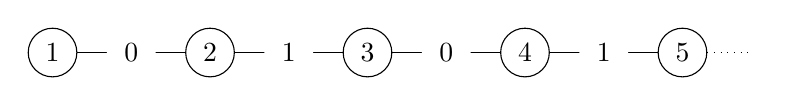
\begin{tikzpicture}

        \begin{scope}[every node/.style={circle,draw}]
          \node (1)  at (0,0)  {1};
          \node (2)  at (2,0)  {2};
          \node (3)  at (4,0)  {3};
          \node (4)  at (6,0)  {4};
          \node (5)  at (8,0)  {5};
        \end{scope}

        \node (6)  at (9,0) {};

        \begin{scope}[every node/.style={fill=white,circle}]

          \begin{scope}[every edge/.style={draw}]
            \path (1)  edge node {$0$} (2);
            \path (2)  edge node {$1$} (3);
            \path (3)  edge node {$0$} (4);
            \path (4)  edge node {$1$} (5);
            \path (5)  edge[style={dotted}] (6);
          \end{scope}
        \end{scope}



      \end{tikzpicture}
      \caption{}
    \end{center}
  \end{figure}

  \paragraph{}
  Une fois ce motif effectué, il faut obligatoirement continuer avec une arête $\rho_2$ et on est dans la même situation que précédement vu qu'il n'y a plus d'arête $\rho_0$ ou $\rho_1$. On rajoute toujours les arêtes par 4 et il est donc impossible d'arriver à 10 arêtes dans le cas du rang 5.

  \paragraph{Rang 4} Pour le rang 4, il nous faut au moins une 4-transposition pour arriver à 10 arêtes. Cette 4-transposition ne peut être $\rho_0$ car nous n'aurions pas assez d'arêtes de $\rho_1$ pour la relier. Il s'agit donc de $\rho_1$ (à la dualité près). Donc nous pouvons appliquer le même raisonnement que celui utilisé pour le rang 5 sur les involutions $\rho_2$ et $\rho_3$. Il faut donc que $\rho_3$ commence et/ou termine le chemin. S'il n'est utilisé qu'à une des deux extrémités, nous obtenons le début de chemin suivant:

  \begin{figure}[H]
    \begin{center}
      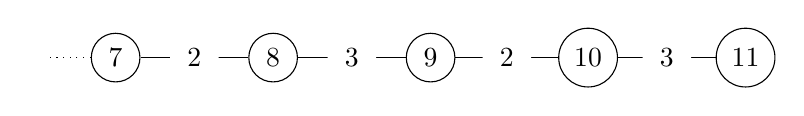
\begin{tikzpicture}

        \begin{scope}[every node/.style={circle,draw}]
          \node (5)  at (0,0)  {7};
          \node (4)  at (2,0)  {8};
          \node (3)  at (4,0)  {9};
          \node (2)  at (6,0)  {10};
          \node (1)  at (8,0)  {11};
        \end{scope}

        \node (6)  at (-1,0) {};

        \begin{scope}[every node/.style={fill=white,circle}]

          \begin{scope}[every edge/.style={draw}]
            \path (1)  edge node {$3$} (2);
            \path (2)  edge node {$2$} (3);
            \path (3)  edge node {$3$} (4);
            \path (4)  edge node {$2$} (5);
            \path (5)  edge[style={dotted}] (6);
          \end{scope}
        \end{scope}

      \end{tikzpicture}
      \caption{}
    \end{center}
  \end{figure}

\paragraph{}
Si nous voulons continuer le chemin, nous devons ajouter les arêtes suivante : $\rho_1, \rho_0, \rho_1, \rho_0, \rho_1$ mais il nous reste une arête $\rho_1$ à la fin. Il faudrait donc que $\rho_3$ commence et termine le graphe. On aurait un début de chemin comme suit:

\begin{figure}[H]
  \begin{center}
    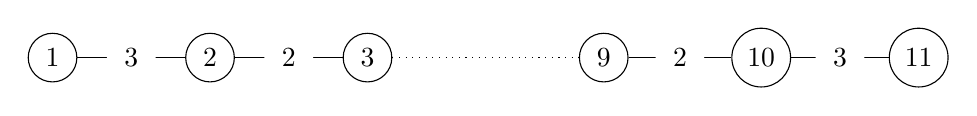
\begin{tikzpicture}

      \begin{scope}[every node/.style={circle,draw}]
        \node (1)  at (0,0)  {1};
        \node (2)  at (2,0)  {2};
        \node (3)  at (4,0)  {3};
        \node (9)  at (7,0)  {9};
        \node (10) at (9,0)  {10};
        \node (11) at (11,0) {11};
      \end{scope}



      \begin{scope}[every node/.style={fill=white,circle}]

        \begin{scope}[every edge/.style={draw}]
          \path (1)  edge node {$3$} (2);
          \path (2)  edge node {$2$} (3);
          \path (3)  edge[style={dotted}] (9);
          \path (9)  edge node {$2$} (10);
          \path (10) edge node {$3$} (11);
        \end{scope}
      \end{scope}

    \end{tikzpicture}
    \caption{}
  \end{center}
\end{figure}

\paragraph{}
Mais si on essaie de compléter les arêtes manquantes, on trouve qu'elle doivent commencer par $\rho_1, \rho_0, \rho_1, \rho_0, \rho_1$ car c'est la seule possibilité mais on ne sait pas placer la dernière arête $\rho_1$.

\end{proof}
